\section{Estruturas de dados}

A fim de se facilitar a programa��o e o entendimento do projeto, foram criadas duas estruturas de dados que s�o acessadas em assembly. A primeira, o Process Control Block � respons�vel pelo armazenamento do estado de um processo. J� a Lista de Threads realiza o controle de quais threads est�o ativas.

\subsection{Process Control Block} \label{sub:PCB}

O Process Control Block (ou simplesmente PCB) � um estrutura de dados que guarda todas as informa��es de uma thread que aguarda para ser executada enquanto outras est�o ativas. H� um PCB para cada uma das nove threads e cada uma ocupa 68 bytes. Ou seja, o espa�o total ocupado pelos PCBs � de 9 $\cdot$ 68 = 612 bytes. Estes 68 bytes est�o estruturados como explicitado na figura \ref{pcb}. Cada posi��o da tabela ocupa uma palavra (4 bytes). A primeira posi��o � em (base do PCB - 4), a segunda em (base do PCB - 8) e assim por diante. Como podemos observar pela figura, as posi��es 1 a 15 ((base do PCB - 4) a (base do PCB - 60)) armazenam o conte�do dos registradores r0 a r14 do modo user em ordem inversa. A posi��o 16 (base do PCB - 64) armazena o link register do modo IRQ, ou seja, o endere�o de retorno da interrup��o. Finalmente, a posi��o 17 armazena o registrador de estado do modo user. Estes registradores armazenados permitem estabelecer um retrato preciso do estado do processo quando houve o chaveamento e permite tamb�m que este estado seja restabelecido quando for o turno deste processo voltar a ser executado. A estrutura tem seu espa�o reservado no arquivo handler\_irq.s, e � nomeado com a vari�vel process\_control\_block, que indica a base da estrutura. Cada um dos PCBs est� logo a seguir do anterior. Por exemplo, a base do primeiro PCB est� em (process\_control\_block - 68), do segundo em (process\_control\_block - 2 $\cdot$ 68) e assim por diante.

\begin{figure}[!ht]
\centering 
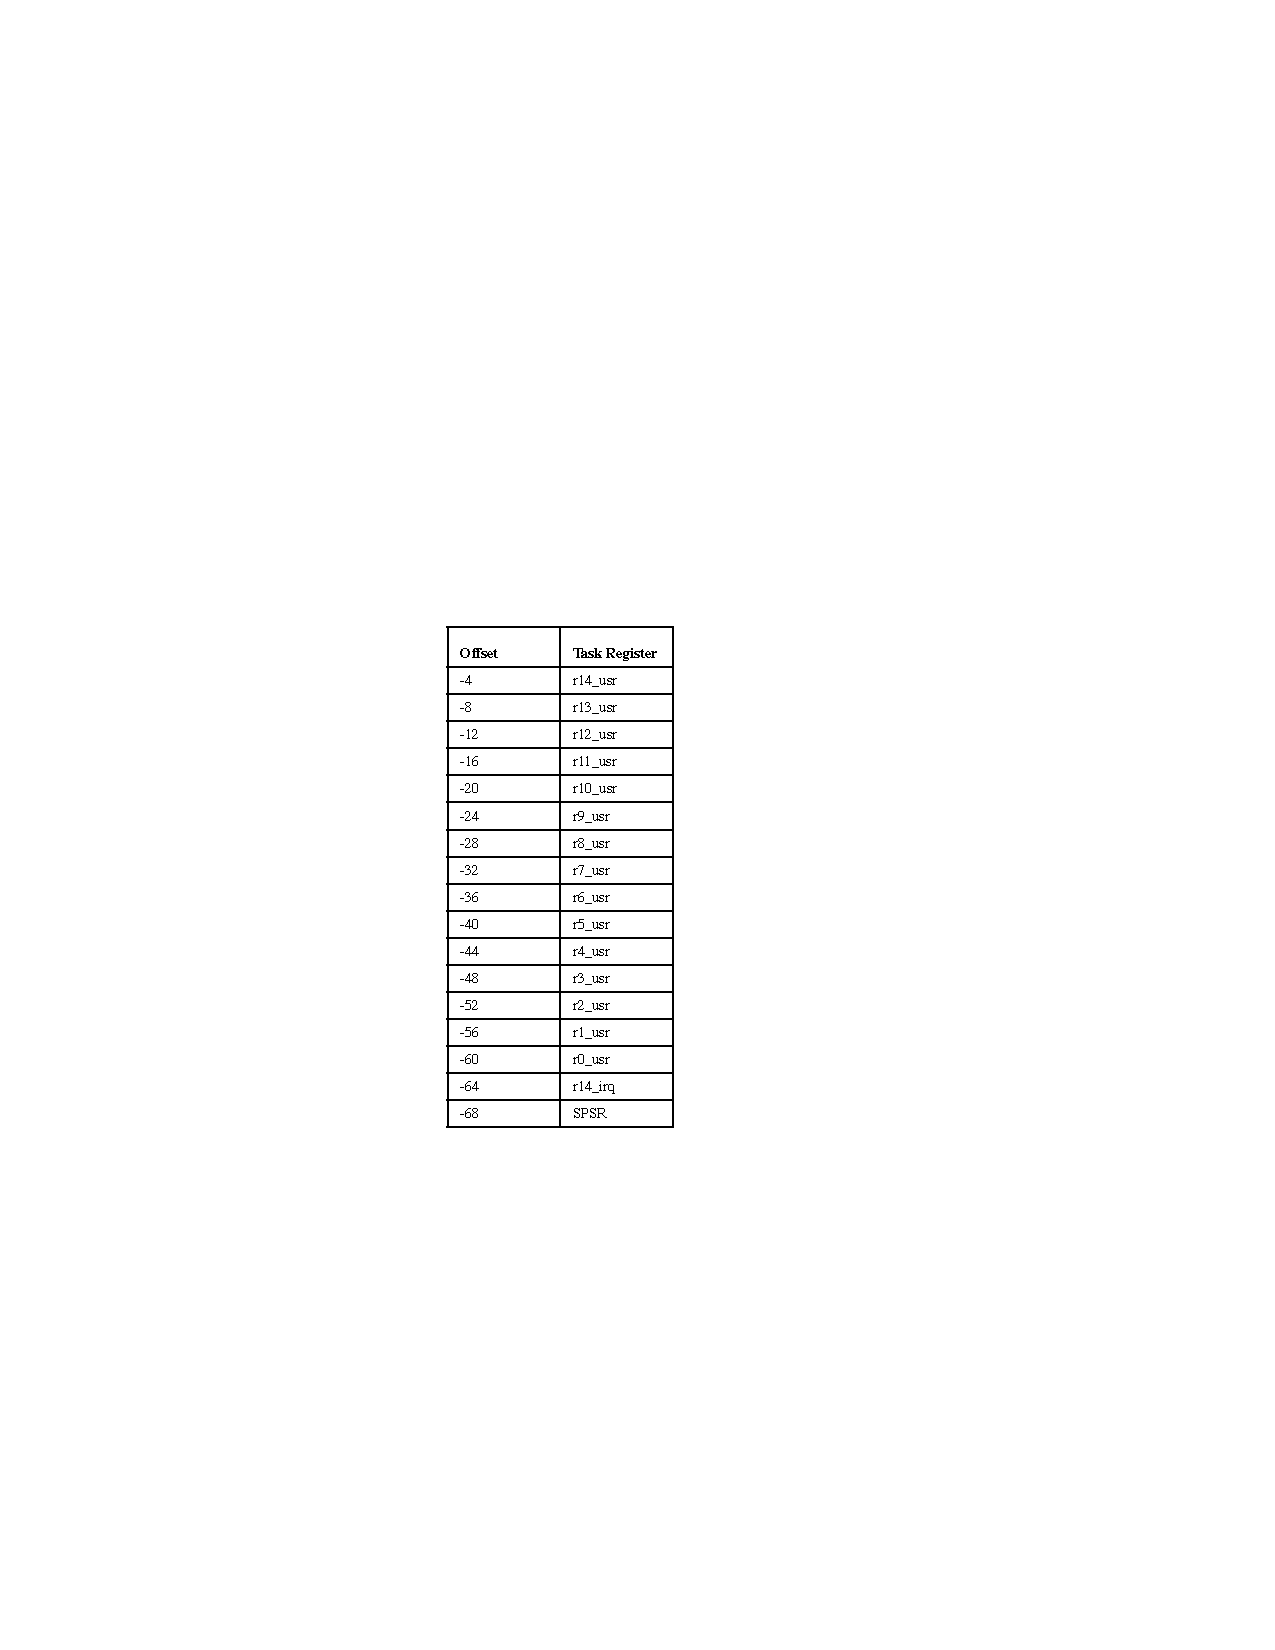
\includegraphics[height=10cm]{figuras/pcb.pdf}
\caption{Estrutura de dados do PCB. Fonte: \cite{Sloss2001} \label{pcb}}
\end{figure}

\subsection{Vetor de threads}

O vetor de threads � uma lista que armazena quais das threads est�o ativas e quais n�o est�o, a fim de se identificar quais devem ser colocadas em execu��o. Cada identificador ocupa 4 bytes, e pode ter os valores 0 (inativo) ou 1 (ativo). Como h� 9 processos, o tamanho deste vetor � de 4 $\cdot$ 9 = 36 bytes. Seu espa�o � reservado no arquivo handler\_irq.s, com o nome de thread\_array. No exemplo na figura \ref{vetor} podemos ver que as threads 1, 2 e 4 est�o ativas, enquanto que as outras n�o est�o.\\

\begin{figure}[!ht]
\centering 
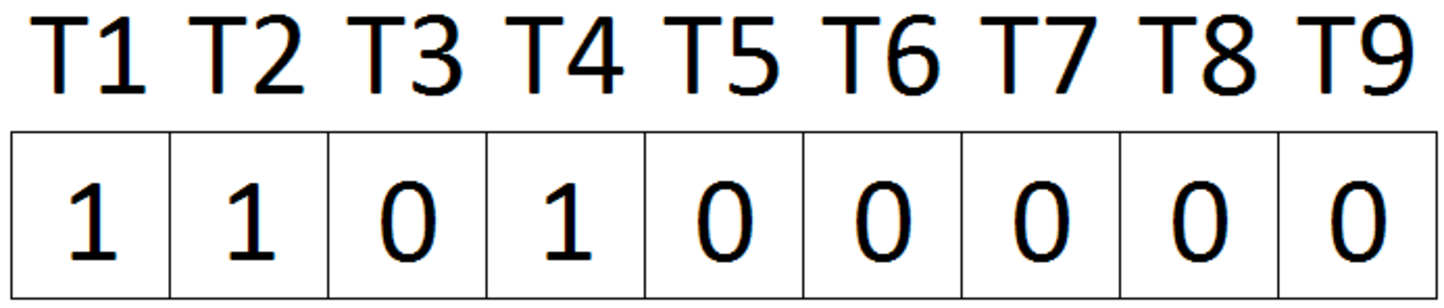
\includegraphics[width=7.5cm]{figuras/vetorThreads.pdf}
\caption{Vetor de threads. \label{vetor}}
\end{figure}